\documentclass{beamer}
\usetheme{CambridgeUS}
\usepackage{amsmath}
\usepackage{amssymb}
\usepackage{tikz}
\usetikzlibrary{arrows.meta, positioning}
\usepackage{cancel}
\usetikzlibrary{positioning}
\usepackage{subcaption}
\usepackage{booktabs}
\usepackage{comment}
\usetikzlibrary{shapes.geometric}
\usepackage{graphicx}

\tikzset{
box/.style={
draw,
rectangle,
rounded corners,
align=left,
font=\small,
inner sep=4pt,
fill=green!15
}
}



\title[On solving the VGLCSP]{On Solving the Multiple Variable Gapped Longest Common Subsequence Problem}

\author[Djukanovic et al.\ \ \ \ \  \ \ \ \ \ \ \ \ \ \ \ \ \ \ \ \ \ \  \ \ \ \ \ \ \ \ \ \ \ \ ]{Marko Djukanović\inst{1,2,6}  \and Nikola Balaban\inst{2}  \and
Christian Blum\inst{3}  \and 
Aleksandar Kartelj\inst{4}  \and
Sašo Džeroski\inst{5}  \and
Žiga Zebec\inst{6}
}
 
\institute{ $^1$University of Nova Gorica, Nova Gorica, Slovenia \\ 
$^2$Faculty of Natural Sciences and Mathematics, University of Banja Luka, Banja Luka, B\&H \\ 
$^3$Artificial Intelligence Research Institute (IIIA-CSIC), Barcelona, Spain \\ 
$^4$Faculty of Mathematics, University of Belgrade, Belgrade, Serbia \\
$^5$Jožef Stefan Institute, Ljubljana, Slovenia \ \\
$^6$Institute of Information Sciences (IZUM), Maribor, Slovenia \\ \vspace{0.3cm}

\footnotesize{-- \textcolor{blue}{EUROCAST 2026: 20th International Conference on Computer Aided Systems Theory, February 23-27, 2026,  Las Palmas de Gran Canaria, Spain}--} \\ \vspace{0.5cm}
\centering

\includegraphics[width=80pt, height=40pt]{SMASH_CMYK-ENG-horizontal_on_white.pdf}~ \hfill
\includegraphics[width=80pt,height=40pt]{IFEEL\_1.png}~\hfill
\includegraphics[width=90pt,height=35pt]{cofunded\_eu.png} ~\hfill
\includegraphics[width=70pt,height=35pt]{slo\_ministry.png}
}%slo_ministry.png

\date{}
\begin{document}
\begin{frame}[plain]
    \maketitle
\end{frame}

%\begin{frame}{Outline}
%    
%    \begin{itemize}
%        \item Introduction  
%         \vspace{0.2cm}
%        \item Problem Definition  \vspace{0.2cm}
%        \item Rooted graph state space  \vspace{0.2cm}
%       \item Iterative multi-source Beam Search  \vspace{0.2cm}
%        \item Experimental Evaluation: General \& special problem
%        \vspace{0.2cm}
%        \item Conclusions
%    \end{itemize}
%\end{frame}
%

\begin{frame}{Introduction}
   \begin{itemize}
       \item Objects we deal with: sequences (strings) over finite alphabet  $\Sigma$
       \begin{itemize}
       \item DNA/RNA over $\{\texttt{A}, \texttt{T}, \texttt{G}, \texttt{C/U}\}$
       \item Proteins over 20 (canonical) amino acids: $\{\texttt{A}, \texttt{C}, \texttt{D}, \texttt{E}, \texttt{P}, \texttt{Q} ...\}$ 
       \end{itemize} \vspace{0.3cm}
        \item \textbf{One of central tasks in computational biology:} 
        \begin{itemize}
        	\item  sequence comparison, finding common motifs between sequences
          \item compare structurally but also semantically/functionality 
          %\item sequence alignment problems 
       \end{itemize} \vspace{0.4cm}
       
       \item \textbf{Subsequences}: reveal structural similarities $\rightarrow$ \textcolor{blue}{\textbf{Longest commmon subsequence problem}} variants (studied 50 years already)
   \end{itemize}
\end{frame}

\begin{frame}{Longest common subsequence problem (LCSP)}
   
    
    \begin{definition}[LCSP]
        \textbf{Input}: Given an arbitrary set of sequences $S=\{s_1, \ldots, s_m\}$ \\
        \textbf{Task}: Find a   subsequence $s$  \textcolor{blue}{common} for all sequences from $S$ with \textcolor{blue}{maximum} possible length ($|s|$). 
    \end{definition} \vspace{0.5cm}
    \begin{example}
       Input: $S=$\{\texttt{\textcolor{red}{A}A\textcolor{red}{T}\textcolor{red}{T}G\textcolor{red}{C}}, \texttt{\textcolor{red}{A}\textcolor{red}{T}\textcolor{red}{T}A\textcolor{red}{C}}\} \\ 
       LCS solution: $s=$\textcolor{red}{ATTC}
    \end{example}
        \vspace{0.3cm}
       % \begin{itemize}
    	%\item Basic problem in computational biology, well-solved  theoretically and practically 
      %\end{itemize}
\end{frame}

\begin{frame}{LCS: Literature \& Problem Variants }
  \begin{itemize}
  \item For $m=2$, polynomially solvable:
  \begin{itemize}
  	   \item  \textcolor{blue}{Dynamic programming}, Hunt-Szymanski, Hirschenberg,  ... 
    \end{itemize} \vspace{0.3cm}
  \item When $m$ arbitrary large -- $\mathcal{NP}$-hard:
   \begin{itemize}
   \item subject of interest over last 30 years -- approximation, meta-heuristic, but also exact approaches   
   \end{itemize}  
  \end{itemize}\vspace{0.5cm}
  
  \textbf{Problem-related practical variants}:
  \begin{itemize}
  		\item Arc-annotated LCS problem, repetition-free, filled LCS problem, ...
  		\item \textcolor{red}{Gapped LCS problem}
  \end{itemize}
\end{frame}

\begin{frame}{The gapped LCS problem (Peng and Yang, 2012)}
   \begin{definition}[A gap sequence]
       Given is a sequence $s$ and an assigned function 
       $G_s \colon \{1, \ldots, |s|\} \mapsto \mathbb{N}$. A pair $(s, G_s)$ is called a {gap sequence}.
   \end{definition} \vspace{0.5cm}
   
   \begin{definition}[A gapped subsequence]
         Sequence $\tilde{s}$ is a \textcolor{red}{gapped subsequence} of $(s, G_s)$ iff 
         \begin{itemize}
             \item $\tilde{s}$ is a subsequence of $s$
             \item the gap constraint $G_s$ fulfilled w.r.t.\ \textit{positions of embedding} (letters of) $\tilde{s}$ in $s$:
         \begin{itemize}
             \item  suppose $i_1< \ldots <i_{|\tilde{s}|}$ are those \textbf{positions}  
             \item ($\forall$ $j=2, \ldots, |\tilde{s}|)\, i_{j} - i_{j-1} \leq G_{s}(i_{j})+1$  (consecutive positions respect gap distances)
         \end{itemize}
       \end{itemize}
   \end{definition}
   
\end{frame}

\begin{frame}{Problem definition}

   \begin{example}
      $s=\texttt{AATTGC}$, $\textcolor{red}{G_s(\cdot)=1}$
      \begin{itemize}
         \item  $\tilde{s}=\texttt{ATG}$, the embedding: \textcolor{red}{A}A\textcolor{red}{T}T\textcolor{red}{G}C (\textcolor{blue}{valid} gapped subsequence)
         \item  $\tilde{s}=\texttt{ATG}$, the embedding: \textcolor{red}{A}A{T}\textcolor{red}{T}\textcolor{red}{G}C (\textcolor{blue}{invalid} gapped subsequence)
      \end{itemize}
   \end{example} \vspace{0.3cm}
    
   \begin{definition}[The multiple (variable) gapped LCS problem -- MVGLCSP]
        \textbf{Input}: Given is a set of gapped sequences $\{ (s_1, G_{s_1}), \ldots, (s_m, G_{s_m}) \}$. \\
        \textbf{Task}: Find the longest  subsequence $\tilde{s}$ so that 
        \begin{itemize}
            \item  $\tilde{s}$ is common subusequence of each $s_i$
            \item $\tilde{s}$ fulfills all gap constraints $G_{s_i}$ ($i=1, \ldots, m$)
        \end{itemize}
    \end{definition}
    \textbf{Note}: when $G_{s_i}=n$ (the length of longest sequence) $\Rightarrow$ VGLCSP = LCSP.
\end{frame}

\begin{frame}{Literature \& Motivation for VGLCSP}
   
   \begin{itemize}
       \item  Peng and Yang (2012, 2014): studied  $m=2$  version by \textbf{three dynamic programming} (DP) approaches (basic and two advanced)
       \item  Manea et al. (2024): complexity analysis investigated
       \item \textcolor{red}{NP-hard} under arbitrary large $m$ 
   \end{itemize} \vspace{0.3cm}
   
   \textbf{Motivation}:
   \begin{itemize}
       \item  \textcolor{blue}{Genetics and molecular biology}: DNA/protein comparison analysis where structural distances between residues must be respected \vspace{0.2cm}
       \item \textcolor{blue}{Time-series analysis}: in settings where events are required to occur within specified temporal delays~(Lainscsek et al. (2015))
   \end{itemize}
   
\end{frame}

\begin{frame}{Methodology}
    \begin{itemize}
        \item Based on the significant extension of the \textbf{state space graph formulation} for LCS problem  (Djukanovic et al. (2020)) \vspace{0.3cm}
        \item \textbf{Gap constraints}: incorporated to cut-off invalid extensions (edges) among the LCS extensions immediately \vspace{0.3cm}
        \item \textcolor{red}{\textbf{Many root/source nodes}} in the state graph (the position of leading letter in a gapped common subsequence free to select)
    \end{itemize}
    
\end{frame}


\begin{frame}{Root-based state graph formulation: rough idea}
  
  
  \begin{itemize}
      
      %\item Start with $p^L=1$, and empty partial solution, refers to the complete problem
      
      \item Each \textbf{state} $v=(p^L, l^v)$: one or more feasible partial solutions where
      \begin{itemize}
      	  \item  a vector of positions $p^L$ refer to the positions of suffixes of input sequences relevant to  further expand these sols (subproblem)
      	  \item the  length of current partial solution $l^v$ 
      \end{itemize}\vspace{0.3cm}
      \item \textbf{Expansion} of $v$: extend (concatenate)  partial solutions feasibly (and non-dominantly) by one letter  in all possible ways,  respecting gap constraints \vspace{0.3cm}
      \item \textbf{Non-expandable nodes}: complete solutions; 
  \end{itemize} \vspace{0.15cm}
  
  \fbox{\textcolor{red}{\textbf{Decision: select appropriate (match)\ $p^L$ for start (empty solution)}}} $\Rightarrow$ possibly \textbf{(exponentially) many root nodes}  \\ \vspace{0.2cm} {Space($p^L$)}: root-based state (sub) graph  induced by root node $(p^L, 0)$.
\end{frame}

\begin{frame}{Root-based state graph formulation: example}
   
    Given $s_1=$\texttt{\fbox{A}BCA},  $s_2=$\texttt{\fbox{A}CAB}, assuming  $G_1=G_2=1$, match $p^L=(1, 1)$; \\ \vspace{0.3cm} \textbf{Space}($(1, 1)$): 
   	
   % U nekom delu LaTeX dokumenta:
   \begin{figure}[h!]
   \centering
   \scalebox{0.55}{
   
   
   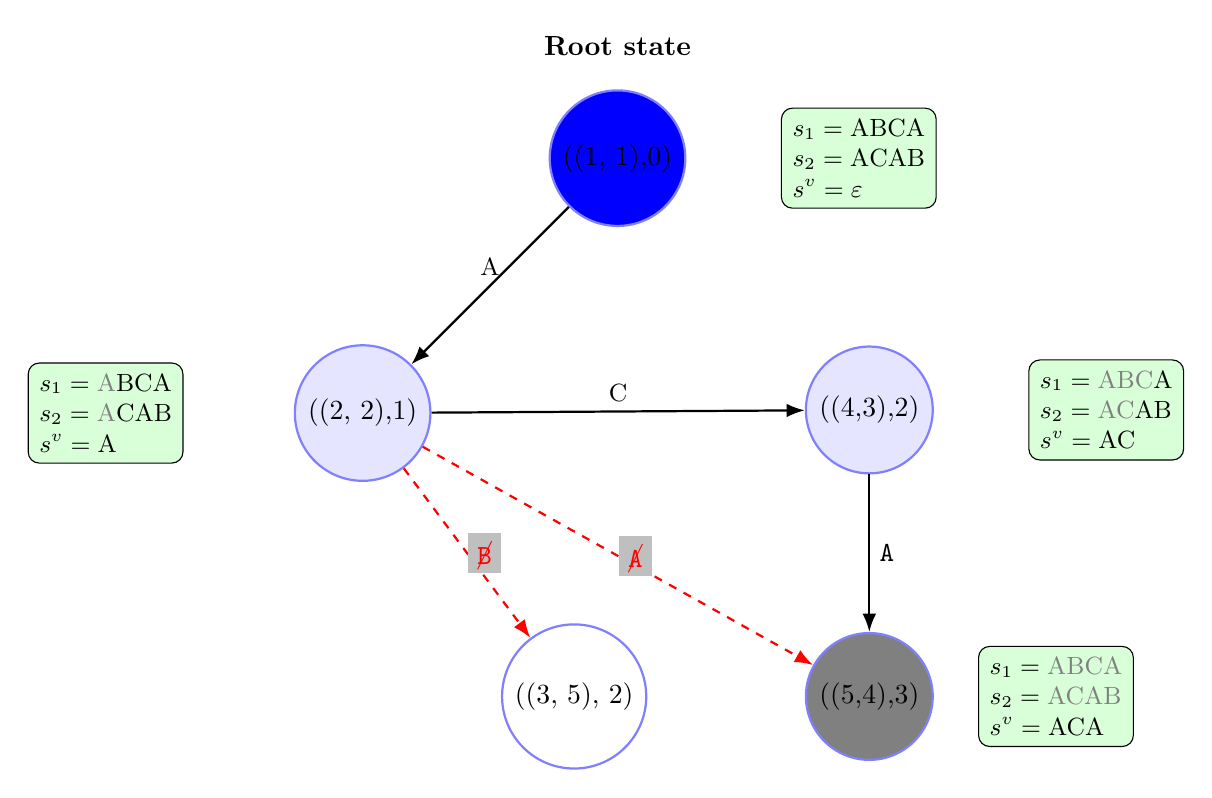
\begin{tikzpicture}[
   state/.style={circle, draw=blue!50, fill=blue!10, thick, minimum size=8mm},
   edge/.style={-Latex, thick},
   node distance=2cm and 2cm
   ]
   
   % Čvorovi
   \node[state, fill=blue] (s0) {((1, 1),0)};
   \node[state, below left=of s0] (s1) {((2, 2),1)};
   \node[state, below right=of s0] (s2) {((4,3),2)};
   %\node[state, below=of s2] (s3) {(4,3)};
   \node[state, below=of s2, fill=gray] (s4) {((5,4),3)}; % krajnje, ali ne koristi se ovde
   \node[state, left=of s4, fill=white] (s5) {((3, 5), 2)}; % krajnje, ali ne koristi se ovde
   
   % Right of root ((1,1),0)
   \node[box, right=12mm of s0] (b0) {
   $s_1=\text{{A}BCA}$\\
   $s_2=\text{{A}CAB}$\\
   $s^v=\varepsilon$
   };
   
   % Left of ((2,2),1)
   \node[box, left=14mm of s1] (b1) {
   $s_1=\text{\textcolor{gray}{A}BCA}$\\
   $s_2=\text{\textcolor{gray}{A}CAB}$\\
   $s^v=\text{A}$
   };
   
   % Right of ((4,3),2)
   \node[box, right=12mm of s2] (b2) {
   $s_1=\text{\textcolor{gray}{ABC}A}$\\
   $s_2=\text{\textcolor{gray}{AC}AB}$\\
   $s^v=\text{AC}$
   };
   
   % Right of ((5,4),3)
   \node[box, right=42mm of s5] (b3) {
   $s_1=\text{\textcolor{gray}{ABCA}}$\\
   $s_2=\text{\textcolor{gray}{ACAB}}$\\
   $s^v=\text{ACA}$
   };
   
 
   
   % Grane (samo validne poklapanja)
   \draw[edge] (s0) -- node[above] {\small A} (s1);
   %\draw[edge] (s0) -- node[above] {\small A} (s2);
   \draw[edge] (s1) -- node[above] {\small C} (s2);
   %\draw[edge] (s2) -- node[right] {\small A} (s3);
   %\draw[edge] (s3) -- node[right] {\texttt{A}} (s4);
   \draw[edge,  scale=2.2, dashed, red] (s1) -- node[right, fill=lightgray] {$\cancel{\texttt{B}}$} (s5);
   
    \draw[edge,  scale=2.2, dashed, red] (s1) -- node[right, fill=lightgray] {$\cancel{\texttt{A}}$} (s4);
   % Oznake
   \node[above=0.3cm of s0] {\textbf{Root state}};
   %\node[below=1.5cm of s3] {\small \textbf{Krajnje stanje}};
   \draw[edge] (s2) -- node[right] {\texttt{A}} (s4);
   
   \end{tikzpicture}}
   
   %\caption{State space graph Space($r=((1, 1), 0)$) for MVGLCSP between the sequences \texttt{\fbox{A}BCA} and  \texttt{\fbox{A}CAB}, assuming $\textcolor{red}{G_1=G_2=1}$.   % \fxnote{Add VGLCS example}
   %}
   
   \label{fig:vgcs-grafstanja}
   \end{figure}
   
\end{frame}


\begin{frame}{An issue with the root-state-space formulation: example}

   \begin{example}
   		$
   		S = \{ s_1 = \texttt{ATGG\fbox{A}AA},\; s_2 = \texttt{ATCC\fbox{A}AA} \},
   		$
   		with $G_{s_1} = G_{s_2} = 1$. 
   		\begin{itemize}
   		     	\item Any state with position vector $\mathbf{p}^L = (5,5)$ \textcolor{red}{cannot be reached} from   $\text{Space}((1,1))$ by standard direct transitions
   		  \end{itemize}

  \end{example} \vspace{0.5cm}
  
   \textbf{Consequence}: $((5, 5), 0) \not \in Space((1, 1))$  $\Rightarrow$  
   \textcolor{blue}{The optimal common subsequence \texttt{AAA} is unreachable} \\ \vspace{0.5cm}%from the basic root $((1,1),0)$,  therefore missed by traditional search strategies.

\textcolor{red}{\textbf{How to fix it?}}
%\vspace{0.5cm}
%   \begin{itemize}
%	    \item The VGLCSP may exhibit multiple, -- potentially exponentially many-- \emph{disconnected root components} 
	   % \item  \textcolor{red}{If started from $(1, 1)$}, it fails to reach    optimal solutions.    
%\end{itemize}
   
\end{frame}

\begin{frame}{Iterative multi-source beam search (IMSBS) strategy}
      
      \begin{itemize}
      	%	\item \textbf{Full state space} of a VGLCSP instance: $\bigcup_{v \in \mathcal{R}} \mathrm{Space}(\mathbf{p}^{L, v})$, with $v=(\mathbf{p}^{L, v}, 0) \in \mathcal{R}$ all root states  
      		\item Explicitly enumerating all root states computationally prohibitive ($O(n^m)$ time) \vspace{0.7cm}
      		\item \textcolor{red}{\textbf{IMSBS}} (rough idea):  \vspace{0.2cm}
      		\begin{itemize}
      		    \item  Exploring \text{Space}($r$): given to \textbf{beam search} --- limited breadth-first-search (BFS) strategy; \textcolor{blue}{parameter $\beta$} controls the number of nodes at each level to be further pursued \vspace{0.2cm}
      		    
      		    \item Dynamically explore multiple promising regions (\text{Space}($\cdot$)) of the state space  \vspace{0.2cm}
      		    \item \textbf{Iteratively identify} a set of \textcolor{red}{promising} candidate root states
      		\end{itemize}
      \end{itemize}  
\end{frame}

\begin{comment}
\begin{frame}{Components and characteristics of IMSBS}
     TODO: Consider not to display this slide!
     
   \begin{itemize}
     	\item $\mathcal{R}$: a \textbf{global set} of root-node candidates, dynamically updated over iterations
     	\item \textbf{Beam search} (\textbf{backward}): not all candidate nodes from $\mathcal{R}$ are root nodes
     	\begin{itemize}
     		\item \textcolor{blue}{\textbf{refine}} them by performing the  {backward} approximate (BS) passes from candidate root nodes to effectively reach distant (real) \textcolor{red}{root node} in the state space
     	\end{itemize}
     	\item  {\textbf{Beam search}} (\textbf{forward}): \textcolor{red}{intensification} in the current root (sub-)space {Space($p$)} -- seek for high-quality (complete) solutions in the corresponding search sub-regions
     	\item \textcolor{red}{diversification}:  during each BS (forward), complete nodes expanded in all possible ways (\textbf{gaps ignored}) to generate candidates for roots (distant from the current region)
     \end{itemize}

\end{frame}
\end{comment}

\begin{frame}{Workflow of the IMSBS}
	%start from the empty source node (0, 0), generating initial (proven) root nodes first -- for each a \in \Sigma => the first occurances of letter a as position p^{L, a} ...   
	 %TODO: draw some plots regarding the workflow of the approach
	 
	 %\begin{figure}[!ht]
	 \centering
	 \scalebox{0.40}{
	 	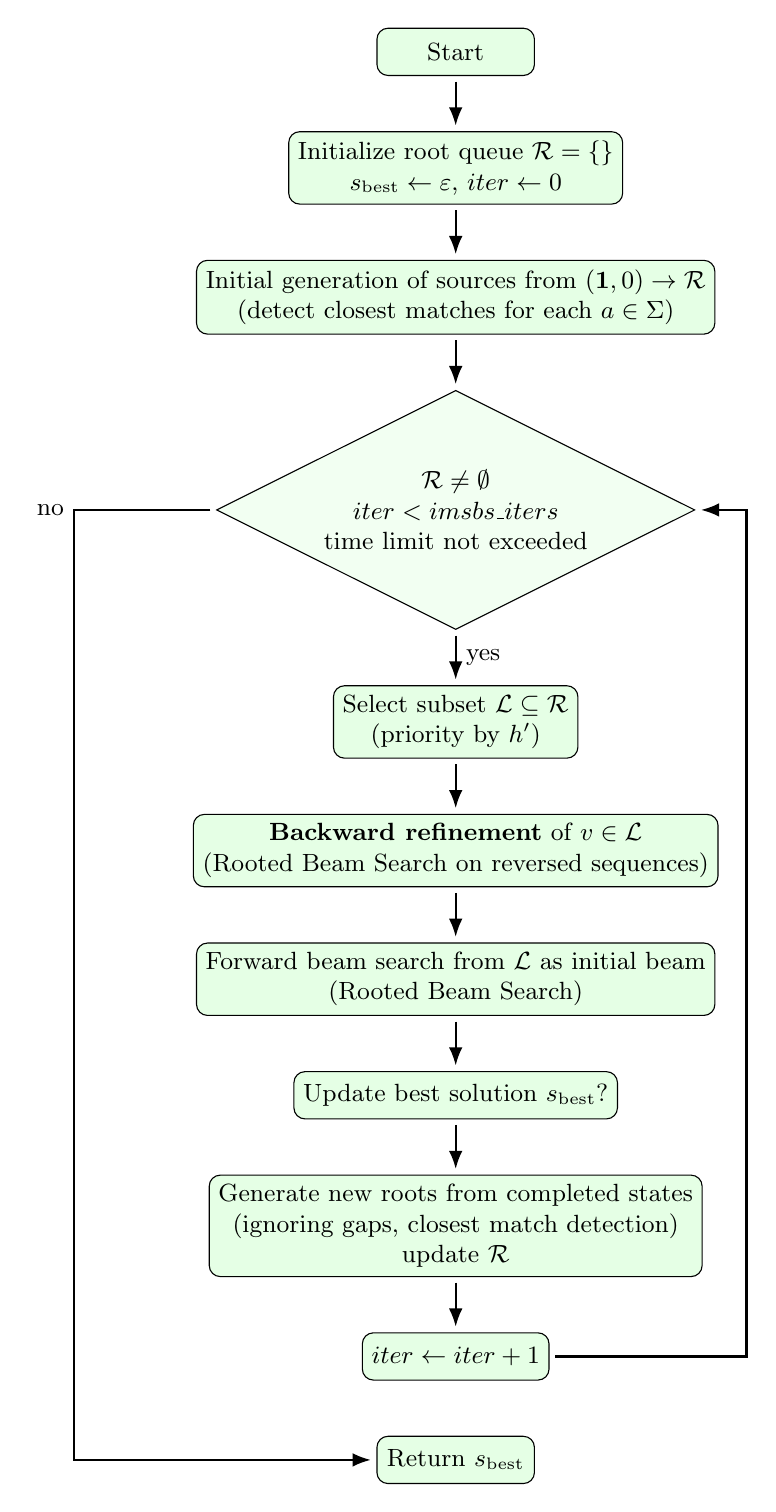
\begin{tikzpicture}[
	 		node distance=0.7cm and 1.2cm,
	 		every node/.style={font=\small},
	 		block/.style={
	 			rectangle,
	 			draw,
	 			rounded corners,
	 			align=center,
	 			minimum width=2.0cm,
	 			minimum height=0.6cm,
	 			fill=green!10
	 		},
	 		decision/.style={
	 			diamond,
	 			draw,
	 			align=center,
	 			aspect=2,
	 			fill=green!5
	 		},
	 		arrow/.style={
	 			->,
	 			thick,
	 			>=Latex,
	 			shorten >=2pt,
	 			shorten <=2pt
	 		}
	 		]
	 		
	 		% Nodes
	 		\node[block] (start) {Start};
	 		
	 		\node[block, below=of start] (init) {Initialize root queue $\mathcal{R}=\{\}$\\
	 			$s_{\text{best}} \leftarrow \varepsilon$, $iter \leftarrow 0$};
	 		
	 		\node[block, below=of init] (expandR) {Initial generation of sources from $(\mathbf{1},0) \rightarrow \mathcal{R}$\\
	 			(detect closest matches for each $a \in \Sigma$)};
	 		
	 		\node[decision, below=of expandR] (while) {$\mathcal{R} \neq \emptyset$\\
	 			$iter < imsbs\_iters$\\
	 			time limit not exceeded};
	 		
	 		\node[block, below=of while] (selectL) {Select subset $\mathcal{L} \subseteq \mathcal{R}$\\
	 			(priority by $h'$)};
	 		
	 		\node[block, below=of selectL] (backward) {\textbf{Backward refinement} of $v \in \mathcal{L}$\\
	 			(Rooted Beam Search on reversed sequences)};
	 		
	 		\node[block, below=of backward] (forward) {Forward beam search from $\mathcal{L}$ as initial beam\\
	 			(Rooted Beam Search)};
	 		
	 		\node[block, below=of forward] (updateBest) {Update best solution $s_{\text{best}}?$};
	 		
	 		\node[block, below=of updateBest] (expandNew) {Generate new roots from completed states\\
	 			(ignoring gaps, closest match detection) \\ update $\mathcal{R}$};
	 		
	 		\node[block, below=of expandNew] (iter) {$iter \leftarrow iter + 1$};
	 		
	 		\node[block, below=of iter] (end) {Return $s_{\text{best}}$};
	 		
	 		% Arrows (main flow)
	 		\draw[arrow] (start) -- (init);
	 		\draw[arrow] (init) -- (expandR);
	 		\draw[arrow] (expandR) -- (while);
	 		
	 		\draw[arrow] (while) -- node[right] {yes} (selectL);
	 		\draw[arrow] (selectL) -- (backward);
	 		\draw[arrow] (backward) -- (forward);
	 		\draw[arrow] (forward) -- (updateBest);
	 		\draw[arrow] (updateBest) -- (expandNew);
	 		\draw[arrow] (expandNew) -- (iter);
	 		
	 		% Explicit loop-back arrow (FIXED)
	 		\draw[arrow]
	 		(iter.east) -- ++(2.5,0)
	 		|- (while.east);
	 		
	 		% Exit arrow
	 		\draw[arrow]
	 		(while.west) -- ++(-1.8,0)
	 		node[left] {no}
	 		|- (end.west);
	 		
	 	\end{tikzpicture}
	 }
	 
	 	%\caption{Simplified workflow of the Iterated Multi-source Beam Search (IMSBS) framework.}
	 	%\label{fig:imsbs_workflow}
	 %\end{figure}
	 
 
\end{frame}

%\begin{frame}{The core advantages of the IMSBS}
% 
%     \begin{itemize}
%     	\item Balance between complete beam search execution (local exploration of promising paths) and the generation of new, promising source nodes (\textcolor{red}{\textbf{global coverage}} of generally weakly-connected search space) \vspace{0.3cm}
%     	\item Preventing from direct suboptimal solutions reduced by employing backward beam search procedure (\textcolor{red}{\textbf{refinement}})
%     \end{itemize}
%      
%\end{frame}

\begin{frame}{Heuristic guidances in BS}
    
    Three LCS heuristic guidances: \vspace{0.2cm}
        \begin{itemize}
       	    \item  $\textrm{UB}_1 $: ``Look-ahead'' for the remaining sequence length
    	    %\begin{equation}
    		%    \textrm{UB}_1(\mathbf{v}) = l^v + \min_{i = 1, \ldots, m} \left( |s_i| - p_i^v + 1 \right)
        	%\end{equation}
        	\vspace{0.3cm}
    	  	\item   $\textrm{UB}_2$: \textit{Character Frequency Alignment} score
    	  	\begin{itemize}
    	  		\item sum up the maximum possible occurrences of each  letters in remaining subsequences
    	  	\end{itemize}
    	   
    	   %\begin{equation}
    	   %	    \textrm{UB}_2(\mathbf{v}) =  l^v + \sum_{\sigma \in \Sigma} 
    	   %	    \min \underbrace{\left( |s_1[p_1^v, |s_1|]|_{\sigma}, \ldots, |s_m[p_m^v, |s_m|]|_{\sigma} \right)}_{\text{remaining valid suffixes}}
    	   %\end{equation}
    	   \vspace{0.3cm}
    	   \item $h_{prob}$: \textit{probability-based heuristic} guidance (matrices of probabilities (Mousavi and Tabataba, 2012)) %These probabilities approximate the probability of the event that a sequence $s$ of length $k$ is a subsequence of a (random) sequence of length $n$ %over an alphabet $\Sigma$.
    \end{itemize}
\end{frame}

\begin{frame}{Experimental Evaluation: arbitrary large $m$-case}
	
	\begin{itemize}
		\item \textsc{Bs}: a baseline beam search, allowing only \textcolor{blue}{a single iteration} of IMSBS (utilizing a huge $\beta$)
 		\vspace{0.3cm}
		\item \textsc{Imsbs-greedy}: fix \textcolor{blue}{beam-width} \( \beta = 1 \) for the forward BS of IMSBS, perform a large number of beam search 
		\begin{itemize}
			\item impact of iterations on the overall performance of \textsc{Imsbs}
		\end{itemize}
	    \vspace{0.3cm}
		\item \textsc{Imsbs}: \textcolor{blue}{a tuned version};  configured to use an average runtime comparable to that of \textsc{Bs}
	\end{itemize}
	
\end{frame}

\begin{frame}{Benchmark set \textsc{Random}}
	 
	 For each combination of instance parameters
	 \begin{itemize}
	 	  \item  $n \in \{50, 100, 200, 500\}$
	 	  \item $m \in \{2, 3, 5, 10\}$
	 	  \item $|\Sigma| \in \{2, 4\}$
	 \end{itemize} 
	 
	 10 random problem instances are generated (sequences uniformly at random). \\ \vspace{0.3cm}
	 
	 Gap constraints generated from $G_{s}(\cdot) \in \mathcal{U}(\{ \lfloor 0.5 \cdot |\Sigma| \rfloor, \ldots, \lfloor 1.5 \cdot |\Sigma| \rfloor \})$.   \\ \vspace{0.7cm}
	 
	 $\Longrightarrow$ A total of \textcolor{red}{\textbf{320 problem instances}} is generated.
	 
\end{frame}

\begin{frame}{Parameter tuning of IMSBS}
	We fixed less sensible params (preliminary tests):
	\begin{itemize}
		\item \textsc{Bs} (backward): $\beta'=10$, and $\textrm{UB}_2$  (efficient)
		\item Candidate root nodes from $\mathcal{R}$ ordered by $\textrm{UB}_2$ (decreasingly)
		\item At each iteration, \textbf{10 best nodes} taken from $\mathcal{R}$ as the initial beam
	\end{itemize} \vspace{0.3cm}
	
\textbf{Tuned parameters:}
	\begin{itemize}
		\item $\beta$ (in BS-forward)
		\item Heuristic guidance in BS (forward)
		\begin{itemize}
			\item $\{\text{UB}_1, \text{UB}_2, h_{prob}\}$
		\end{itemize}
	\end{itemize} \vspace{0.5cm}
	
  \textcolor{red}{\textbf{Grid search used to tune; avg. solution quality over all (320) instances!}}

\end{frame}

\begin{frame}{The results of tuning}%{$\textsc{Bs}$: influence of different $\beta$ and heuristic guidances}
	
	   %\begin{figure}[!ht]
	  	%\centering
	  	%\begin{subfigure}[t]{0.48\textwidth}
	  		%\centering
	  		%\scalebox{0.75}{
	  		%\includegraphics[width=\linewidth, height=140pt]{figures/bs_tuning_quality.png}}
	  		%\caption{Avg. quality over all instances from the %\textsc{Random} benchmark suite.}
	      %\label{fig:tune_bs}
	  	%\end{subfigure}
	  %	~
	  %	\begin{subfigure}[t]{0.48\textwidth}
	  %		\centering
	  %		\includegraphics[width=\linewidth, height=120pt]{figures/bs_tuning_time.png}
	  %		\caption{Avg. runtime over all instances from the \textsc{Random} benchmark suite.}
	  %		\label{fig:tune_bs_time}
	  %	\end{subfigure}
	  %	\caption{Beam search tuning results on the \textsc{Random} benchmark suite.}
	  %\label{fig:bs_tuning}
	  %\end{figure}
	\begin{itemize}
		\item  $ \textbf{\text{(Baseline)}}\ \textsc{Bs} \Longrightarrow  \textcolor{red}{\beta = 10,000}$ and $\textcolor{red}{h = h_{\text{prob}}}$
	    \vspace{0.3cm}
	    \item $ {\textsc{Imsbs}} \Longrightarrow \textcolor{red}{h = \textrm{UB}_2}$,  $\textcolor{red}{\beta = 500},$ and $\textcolor{red}{imsbs\_iter = 100}$ \\ \vspace{0.3cm}
	    \item {\textsc{Imsbs-Greedy}}:  $\textcolor{red}{\beta=1}$, $\textcolor{red}{imsbs\_iter=10,000}$ %(comparable or a bit larger avg. runtime to that of \textsc{Imsbs})
   \end{itemize} 
\end{frame}

%\begin{frame}{Parameter tuning of \textsc{Imsbs}}
	
%	 \begin{figure}[!h]
%		\centering
		%\begin{minipage}{0.48\textwidth}
%		\scalebox{0.7}{
%			\includegraphics[width=\linewidth]{figures/imsbs_tuning.png}}
%			\caption*{Avg. quality for different IMSBS settings over all instances from the \textsc{Random} benchmark suite.}
%			\label{fig:tune_imsbs}
		%\end{minipage}
	%	~
	%	\begin{minipage}{0.48\textwidth}
	%		\centering
	%		\includegraphics[width=\linewidth]{figures/imsbs_tuning_time.png}
	%		\caption*{(b) Avg. runtime for different IMSBS settings over all instances from the \textsc{Random} benchmark suite.}
	%		\label{fig:tune_imsbs_time}
	%	\end{minipage}
		%\caption{IMSBS parameter tuning results on the \textsc{Random} benchmark suite.}
		%\label{fig:imsbs_tuning}
%	\end{figure}
	

%\end{frame}
       
\begin{comment}
	\begin{table}[H]
		%\caption{Numerical results on the \textsc{Random} benchmark suite. }\label{tab:numerical_results_general_m}
		\centering
		\scalebox{0.4}{
			\begin{tabular}{lll|rr|rr|rr}
				\hline
				\multicolumn{3}{c}{Inst.} & \multicolumn{2}{c}{\textsc{Bs}} & \multicolumn{2}{c}{\textsc{Imsbs-Greedy}} & \multicolumn{2}{c}{\textsc{Imsbs}} \\
				\cmidrule(lrr){1-3} \cmidrule(lr){4-5} \cmidrule(lr){6-7} \cmidrule(lr){8-9} \\ 
				$m$ & $n$ & $|\Sigma|$ & $\overline{obj}$ & $\overline{t}[s]$ & $\overline{obj}$ & $\overline{t}[s]$ & $\overline{obj}$ & $\overline{t}[s]$ \\
				\hline
				\midrule
				2 &       50 &         2 &            33.6 &         0.02 &                     33.1 &                  0.00 &         \textbf{37.7} &      0.06 \\
				2 &       50 &         4 &            30.1 &         0.98 &                     27.7 &                  0.00 &         \textbf{30.1} &      0.16 \\
				2 &      100 &         2 &            48.9 &         2.07 &                     64.5 &                  0.01 &         \textbf{72.8} &      0.94 \\
				2 &      100 &         4 &            \textbf{62.1} &        11.19 &                     56.9 &                  0.01 &         61.6 &      0.91 \\
				2 &      200 &         2 &            99.1 &        18.56 &                     95.5 &                  0.02 &        \textbf{136.4} &      6.21 \\
				2 &      200 &         4 &           120.5 &        38.15 &                    116.1 &                  0.05 &        \textbf{124.9} &      6.58 \\
				2 &      500 &         2 &            65.3 &        23.27 &                    153.6 &                  0.07 &        \textbf{265.7} &    119.75 \\
				2 &      500 &         4 &           214.6 &       163.69 &                    227.7 &                  0.12 &        \textbf{294.4} &     60.49 \\ \hline
				3 &       50 &         2 &            17.5 &         0.03 &                     27.2 &                  0.00 &         \textbf{31.2} &      0.14 \\
				3 &       50 &         4 &            21.7 &         0.18 &                     21.5 &                  0.00 &         \textbf{22.9} &      0.19 \\
				3 &      100 &         2 &            19.7 &         0.06 &                     41.8 &                  0.01 &         \textbf{58.5} &      3.15 \\
				3 &      100 &         4 &            34.1 &         2.35 &                     43.4 &                  0.03 &         \textbf{48.4} &      5.58 \\
				3 &      200 &         2 &            15.2 &         0.16 &                     63.6 &                  0.02 &         \textbf{90.0} &     22.48 \\
				3 &      200 &         4 &            85.3 &        23.45 &                     77.2 &                  0.08 &         \textbf{97.1} &     72.25 \\
				3 &      500 &         2 &            12.6 &         0.10 &                     69.9 &                  0.07 &        \textbf{102.9} &     53.56 \\
				3 &      500 &         4 &            90.7 &        86.35 &                    104.2 &                  0.29 &        \textbf{187.7} &    412.27 \\ \hline
				5 &       50 &         2 &             4.8 &         0.00 &                     14.9 &                  0.00 &         \textbf{20.0} &      0.36 \\
				5 &       50 &         4 &             8.9 &         0.01 &                     13.6 &                  0.06 &         \textbf{15.3} &      0.79 \\
				5 &      100 &         2 &             6.3 &         0.01 &                     17.7 &                  0.01 &         \textbf{22.4} &      0.57 \\
				5 &      100 &         4 &             5.3 &         0.01 &                     \textbf{23.2} &                 10.85 &         22.1 &      1.44 \\
				5 &      200 &         2 &             5.3 &         0.01 &                     21.6 &                  0.03 &         \textbf{26.6} &      1.07 \\
				5 &      200 &         4 &             6.4 &         0.02 &                     \textbf{32.5} &                604.11 &         {25.7} &      2.10 \\
				5 &      500 &         2 &             5.9 &         0.10 &                     25.5 &                  0.14 &         \textbf{27.9} &      3.22 \\
				5 &      500 &         4 &             6.8 &         0.10 &                     \textbf{43.6} &               1341.25 &         26.9 &      3.52 \\ \hline
				10 &       50 &         2 &             1.7 &         0.00 &                      8.8 &                  2.28 &          \textbf{9.1} &      0.47 \\ 
				10 &       50 &         4 &             1.9 &         0.00 &                      \textbf{7.0} &                508.36 &          6.1 &      1.46 \\
				10 &      100 &         2 &             1.1 &         0.00 &                     \textbf{14.0} &               1421.10 &          8.6 &      0.54 \\
				10 &      100 &         4 &             2.2 &         0.01 &                      \textbf{8.9} &               1800.45 &          {6.3} &      1.51 \\
				10 &      200 &         2 &             2.5 &         0.01 &                     \textbf{13.2} &               1710.49 &         10.3 &      0.77 \\
				10 &      200 &         4 &             2.2 &         0.02 &                      \textbf{7.9} &               1800.54 &          6.1 &      1.74 \\
				10 &      500 &         2 &             1.8 &         0.08 &                     \textbf{13.8} &               1611.70 &          {9.5} &      1.53 \\
				10 &      500 &         4 &             1.9 &         0.09 &                      \textbf{8.2} &               1800.46 &          6.1 &      2.37 \\
				\hline \hline
				\textbf{Avg.} &  &  &  32.38 & 10.97 & 46.82 & 394.14 &  \textbf{59.73} & 24.63  \\ \hline \hline
		\end{tabular}}
	\end{table}
\end{comment}  

\begin{frame}{Numerical results}
	
	%res_general_m2.png, res_general_m3.png, res_general_m5.png, res_general_m10.png
   \centering
   \begin{columns}[T]
   	\begin{column}{0.5\textwidth}
   		\centering
   		\textbf{$\footnotesize{m=2}$}\\ 
   		\includegraphics[width=150pt,height=90pt]{figures/res_general\_m2.png}
   		
   		
   		\textbf{$m=5$}\\ 
   		\includegraphics[width=150pt,height=90pt]{figures/res_general\_m5.png}
   	\end{column}
   	
   	\begin{column}{0.5\textwidth}
   		\centering
   		\textbf{$\footnotesize{m=3}$}\\ 
   		\includegraphics[width=150pt,height=90pt]{figures/res_general\_m3.png}
   		
   		\textbf{$\footnotesize{m=10}$}\\ 
   		\includegraphics[width=150pt,height=90pt]{figures/res_general\_m10.png}
   	\end{column}
   \end{columns}
 
\end{frame}

\begin{comment}
	

\begin{frame}{Numerical results for $m=2$ case}
	    
	  \begin{itemize}
	 	  \item \textsc{Dp}-1: the basic DP $(O(n^2m^2))$ \vspace{0.2cm}
	 	  \item \textsc{Dp}-2: an advanced DP, uses Incremental Suffix Maximum Queries (ISMQ) --- \texttt{Col} and \texttt{All} matrices %the basic DP algorithm
	 	     $(O(n^2 + mn))$  \vspace{0.2cm}
	 	    \item \textsc{Dp}-3: an enhanced DP --- ISMQ handled  with a \textit{deque} structure %for further speedup 
	 	    (slightly modified w.r.t.\ the literature) \vspace{0.2cm}
	 	    \item \textsc{Ilp}: an integer linear programming, \textbf{proposed in this work}, motivated by the ILP model for LCSP %with $m=2$
	 \end{itemize} \vspace{0.5cm}
\textcolor{blue}{\textbf{The first known empirical study for the $m=2$} (80 instances).}
\end{frame}
\end{comment}


\begin{frame}{Numerical results for $m=2$}
	
	\begin{figure}
		\includegraphics[width=240pt,height=150pt]{figures/results\_m\_eq\_2.png}
	\end{figure}
	
 
\begin{itemize}
	\item \textcolor{blue}{\textbf{The first known empirical study for the $m=2$} (80 instances)}
	\item \textsc{Ilp}: proposed in this work  
\end{itemize}
	 
\end{frame}

\begin{comment}
	\begin{table}[H]
		\caption{Results on the \textsc{Random} benchmark set for $m=2$: the exact approaches from the literature.}\label{tab:results-2d-literature}
		\centering
		\scalebox{0.7}{
			\begin{tabular}{lll|lr|rr|rr|rr}
				\hline
				\multicolumn{3}{c}{Inst.} & \multicolumn{2}{c}{\textsc{Dp}-1}  &
				\multicolumn{2}{c}{\textsc{Dp}-2} & \multicolumn{2}{c}{\textsc{Dp}-3} & 
				\multicolumn{2}{c}{\textsc{Ilp}}  \\
				\cmidrule(lrr){1-3} \cmidrule(lr){4-5}
				\cmidrule(lr){6-7} \cmidrule(lr){8-9}
				\cmidrule(lr){10-11} 	\\ 
				$m$ & $n$ & $|\Sigma|$ & $\overline{obj}$ & $\overline{t}[s]$ & $\overline{obj}$  & $\overline{t}[s]$ &$\overline{obj}$  & $\overline{t}[s]$ & $\overline{obj}$  & $\overline{t}[s]$ \\
				\hline
				2 &   50 &         2 &              38.1 &          0.01 & 38.1 &          \textbf{0.01} &              38.1 &          0.01  & 38.1 & 168.3 \\
				2 &   50 &         4 &              30.3 &          \textbf{0.01} &              30.3 &          0.02 &              30.3 &          0.02 & 30.3  & 28.0 \\ \hline
				2 &  100 &         2 &              77.4 &          0.1 &              77.4 &          \textbf{0.03} &              77.4 &          0.05 & -- & -- \\
				2 &  100 &         4 &              62.3 &          0.07 &              62.3 &         \textbf{0.06} &              62.3 &          0.09 & 0.00 & 1800.0 \\ \hline
				
				2 &  200 &         2 &             156.4 &          0.75 &             156.4 &          \textbf{0.13} &             156.4 &          0.16  & -- & -- \\
				2 &  200 &         4 &             127.2 &          0.59 &             127.2 &          \textbf{0.25} &             127.2 &          0.32  & -- & -- \\ \hline
				
				2 &  500 &         2 &             395.9 &         13.57 &             395.9 &          \textbf{0.84}  &             395.9 &          1.05 & -- & -- \\
				2 &  500 &         4 &             317.2 &         10.18 &             317.2 &          \textbf{1.70} & 317.2 &  2.1 & -- &-- \\    
				\hline \hline
		\end{tabular}}
		
	\end{table} 
	
\end{comment}


\begin{frame}{The $m=2$ case: heuristic performance vs. optimal solution }
	
  \begin{figure}[htbp]
	%	\centering
	%	\begin{minipage}{0.48\textwidth}
	%		\includegraphics[width=\linewidth]{figures/bs_imsbs_imbs_greedy_vs_dp_quality_distribution.png} 
	%		\caption*{(a) Relative solution quality percentage distribution for each heuristic approach with respect to the optimal solutions.} 
	%	\end{minipage}
	%	\hfill
	%	\begin{minipage}{0.48\textwidth}
			\centering
			\includegraphics[width=320pt,height=160pt]{figures/bs_imsbs_imsbs_greedy_vs_dp_quality.png}
			\caption*{ Relative solution quality achieved by the heuristic approaches compared to the optimal solutions (shown in \%).}
		%\end{minipage}
		%\caption{Number of instances for which \textsc{Bs} and \textsc{Imsbs} achieve a specific ratio of the obtained (approximate) solution quality to the known optimal solution for $m=2$.}
		%\label{fig:optimal-vs-heuristic}
	\end{figure}
	
	
 \end{frame}

\begin{frame}{Conclusions and Future Work}
	
	\begin{itemize}
		\item Proposed a \textcolor{red}{\textbf{general heuristic framework}} IMSBS to solve the multiple VGLCS problem  
		\item Combines consecutive Beam search calls which induce refinement of sources, source node generation for further  iterations
		\begin{itemize}
			\item  balance between intensification and diversification 
	    \end{itemize}
		\item Empirical studies conducted for the first time on the \textcolor{red}{\textbf{synthetic instances}}: IMSBS outperforms the baseline Beam search  
	\end{itemize}    \vspace{0.3cm}
	
\textbf{Future work:}
	\begin{itemize}
		\item \textcolor{red}{\textbf{Real-world}} instance-case scenario
		\item Lack of more advanced heuristic guidance: \textcolor{red}{\textbf{Data-driven/ML heuristic}} involving various local and global features (NN-based)
	\end{itemize}
\end{frame}

\begin{frame}
	
	\centering
	\Large{\textcolor{blue}{\textbf{Thank you for your attention!}}}
	
\end{frame}


\end{document}
